%==============================================================================
% Quantitative Modeling and Analysis (QMA)
%
% FMT, UTwente
%==============================================================================

\documentclass{beamer}

%==============================================================================
%color theme
%==============================================================================

%beamer theme and color
\usetheme{ut}

%==============================================================================
%packages
%==============================================================================

%\usepackage{beamerthemeshadow}
\usepackage[english]{babel}
\usepackage[utf8]{inputenc}
\usepackage{tikz}
\usepackage{multirow}
\usepackage{color, colortbl}
\usepackage{subfigure}
\usepackage{amsmath}

\usepackage{listings}

\usetikzlibrary{arrows,shapes,snakes,automata,backgrounds,petri}
\tikzstyle{every picture}+=[shorten <=0pt, inner sep=2pt, auto, font=\tiny]
\tikzstyle{initial}+=[initial text=]
\tikzstyle{every state}+=[minimum size=3mm, node distance=4cm]
\tikzstyle{dot}=[circle,thick,minimum size=0.5mm,fill=black, inner sep=1pt]

\setbeamercovered{transparent=10} % of transparency

%\bibliographystyle{abbrv}

%==============================================================================
%language
%==============================================================================

\selectlanguage{english}

%==============================================================================

\beamertemplatenavigationsymbolsempty

%========================================================================================
% Custom commands
%========================================================================================


%==============================================================================
%Titel
%==============================================================================

\title[QMA - Exponential distributions]{Quantitative Modeling and Analysis}
\subtitle{Lecture: Exponential distributions}
\author[FMT]{Florian Arnold, Dennis Guck and Gerjan Stokkink}
\institute[EWI-FMT]{Formal Methods and Tools Group,\\ University of Twente}
\footlinetext{QMA - Exponential distributions}
\date{}

%==============================================================================
%LaTeX code
%==============================================================================

\begin{document}

\begin{frame}
\titlepage
\end{frame} 

%==============================================================================
%Inhaltsverzeichnis
%==============================================================================

\begin{chapterframe}
	\chaptertitle{Overview}
	\tableofcontents[subsectionstyle=hide]
\end{chapterframe}

%==============================================================================
\section{Geometric distribution}
%==============================================================================

\begin{chapterframe}
	\chaptertitle{Overview}
	\tableofcontents[currentsection,subsectionstyle=hide]
\end{chapterframe}

\subsection{Geometric distribution}

\begin{frame}
	\frametitle{Geometric distribution}
	\begin{block}{Geometric distribution}
	\begin{figure}
        \centering
        \subfigure[pdf]{\label{subfig:geopdf}
	        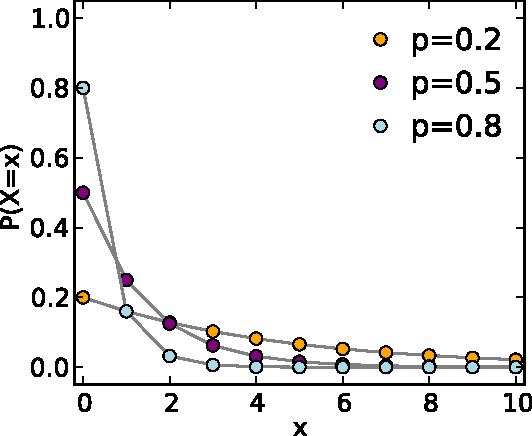
\includegraphics[width=0.4\textwidth]{img/geo_pdf.pdf}
		}
		\subfigure[cdf]{\label{subfig:geocdf}
			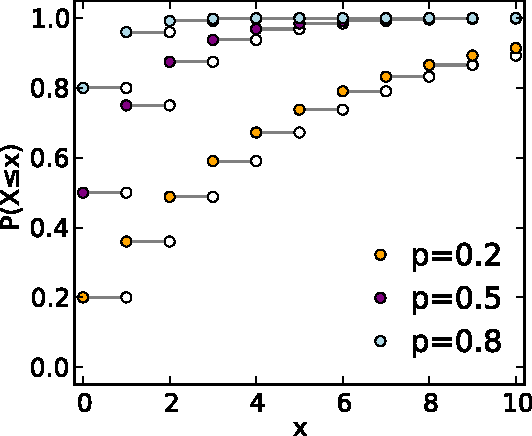
\includegraphics[width=0.4\textwidth]{img/geo_cdf.pdf}
		}
        %\caption{Geometric distribution.}\label{fig:geom}
	\end{figure}
	\end{block}
\end{frame}

%==============================================================================
\section{Exponential distribution}
%==============================================================================

\begin{chapterframe}
	\chaptertitle{Overview}
	\tableofcontents[currentsection,subsectionstyle=hide]
\end{chapterframe}

\subsection{Negative exponential distribution}

\begin{frame}
	\frametitle{Continuous random variables}
	\begin{itemize}
		\item $X$ is a random variable (short r.v.)
			\begin{itemize}
				\item on a sample space with probability measure $Pr$ (Lebesgue measure)
			\end{itemize}
		\item $X$ is \textcolor{utblue}{continuously distributed} if there exists a function $f(x)$ such that:
			{\small
			\begin{equation*}
				F_x(d)=Pr\{X\geq d\}=\int_{-\infty}^{d}f(x)dx
			\end{equation*}
			for each $d\in\mathbb{R}$ where $F$ satisfies: $f(x)\geq 0$ for all $x$ and 
			\begin{equation*}
				\int_{-\infty}^{\infty}f(x)dx=1.
			\end{equation*}}
	\end{itemize}
\end{frame}

\begin{frame}
	\frametitle{Negative exponential distribution}
	\begin{block}{Exponential distribution}
	\begin{figure}
        \centering
        \subfigure[pdf]{\label{subfig:exppdf}
	        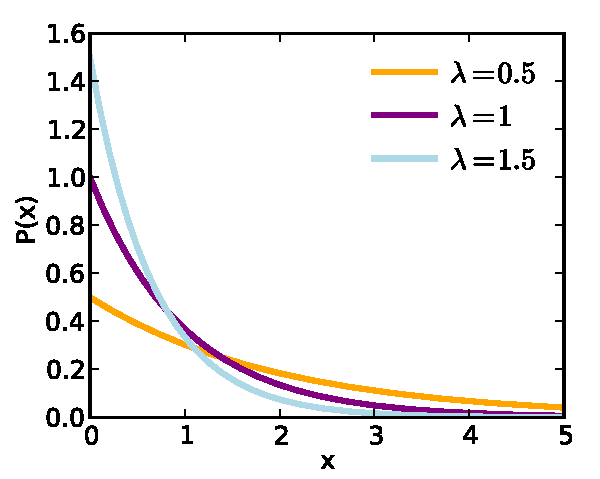
\includegraphics[width=0.4\textwidth]{img/exp_pdf.pdf}
		}
		\subfigure[cdf]{\label{subfig:expcdf}
			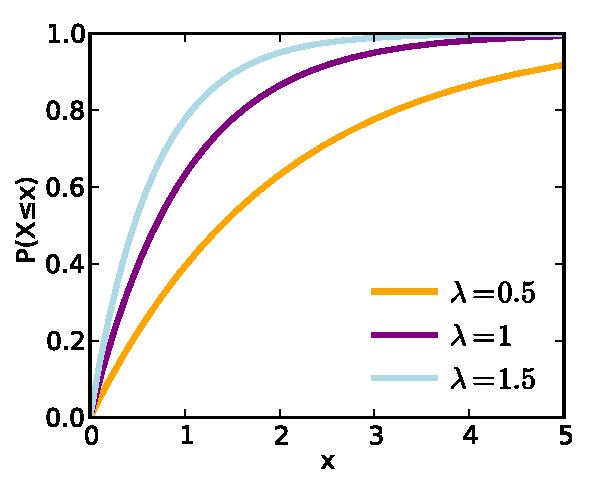
\includegraphics[width=0.4\textwidth]{img/exp_cdf.pdf}
		}
        %\caption{Geometric distribution.}\label{fig:geom}
	\end{figure}
	\end{block}
\end{frame}

\begin{frame}
	\frametitle{Memoryless property}
	\begin{block}{Theorem}
		Let $X$ be a exponential distributed r.v., then: 
		\begin{equation*}
			Pr\{X > t + d | X > t\} = Pr\{X > d\} \text{ for any } t, d\in\mathbb{R}_{\geq 0}.
		\end{equation*}
	\end{block}
	\vspace{2ex}
	%Proof on the blackboard.
	\onslide<2>{
	{\small
	\textit{Proof}: Let $\lambda$ be the rate of $X$'s distribution. Then we derive:
	\begin{eqnarray*}
		Pr\{X>t+d|X>t\} & = & \frac{Pr\{X>t+d \cap X>t\}}{Pr\{X>t\}} = \frac{Pr\{X>t+d\}}{Pr\{X>t\}}\\
		 = \frac{e^{-\lambda\cdot(t+d)}}{e^{-\lambda\cdot t}} & = & e^{-\lambda\cdot d} = Pr\{X>d\}.
	\end{eqnarray*}}}
	\vspace{2ex}
	\let\thefootnote\relax\footnote{Note: Any cdf which is memoryless is a negative exponential one.}
\end{frame}

\end{document}

